\chapter{Gierer-Meinhardt Model}

In this chapter, we introduce two fixed time delay variants of the Gierer-Meinhardt (GM) model. Through a similar linear analysis to that in Chapter \ref{section:fixdel} considered for the LI variant of the Schnakenberg model, we look to examine the effect of an increasing time delay on the Turing space for the GM model. The model descriptions we use here are motivated by the analysis conducted in \cite{fadai1,fadai2}. The spike solution analysis in \cite{fadai1,fadai2} suggest that the placement of time-delayed terms in the model is of extreme importance in the context of pattern formation. A chemical interpretation of the kinetic reactions for the GM Model can be found in \cite{leegaffmonk}. The two non-dimensionalised model descriptions we consider, with kinetic reactions taken from \cite{murray}, and time-delayed terms motivated by \cite{fadai1} and \cite{fadai2}, are given by \eqref{fadai1} and \eqref{fadai2} respectively.
\begin{multicols}{2}
\begin{equation}\label{fadai1}
  \left.\begin{split}
\frac{\partial u}{\partial t}&=\frac{\epsilon^2}{L^2}\frac{\partial^2 u}{\partial x^2}+a-bu+\frac{\hat{u}^2}{\hat{v}}\\
\frac{\partial v}{\partial t}&=\frac{1}{L^2}\frac{\partial^2 v}{\partial x^2}+\hat{u}^2-v,
\end{split}\right\}
\end{equation}
\break
\begin{equation}\label{fadai2}
  \left.\begin{split}
\frac{\partial u}{\partial t}&=\frac{\epsilon^2}{L^2}\frac{\partial^2 u}{\partial x^2}+a-bu+\frac{\hat{u}^2}{v}\\
\frac{\partial v}{\partial t}&=\frac{1}{L^2}\frac{\partial^2 v}{\partial x^2}+\hat{u}^2-v.
\end{split}\right\}
\end{equation}
\end{multicols}
We note the difference in the two models being the $v$ term in the activator's kinetics. The notation $\hat{u}$ and $\hat{v}$ denote the activator and inhibitor evaluated at some fixed time delay $\tau$, namely $\hat{u}=u(x,t-\tau)$, $\hat{v}=v(x,t-\tau)$. The results in \cite{fadai1,fadai2} showed that an increasing time delay in \eqref{fadai1} acted as a de-stabilising agent, and shrunk the parameter space exhibiting stable spike solutions. In contrast, an increasing time delay incorporated as in \eqref{fadai2} caused an expansion of the stable spike solution parameter regime. In this chapter, we use linear analysis of the spatially homogeneous steady states to examine how an increasing time delay will affect the Turing space seen for each of these variants. Figure \ref{fig:gmspace} shows the stable and unstable parameter regimes as well as the Turing space for a $\tau=0$. The parameter space considered is $(a,b)\in[0,1]\times[0,4]$, and the steady state for the GM model is given as $(u_\star,v_\star)=\left(\frac{a+1}{b},\left(\frac{a+1}{b}\right)^2\right)$.

\begin{figure}[H]
    \centering
    \begin{subfigure}[t]{0.45\textwidth}
        \centering
        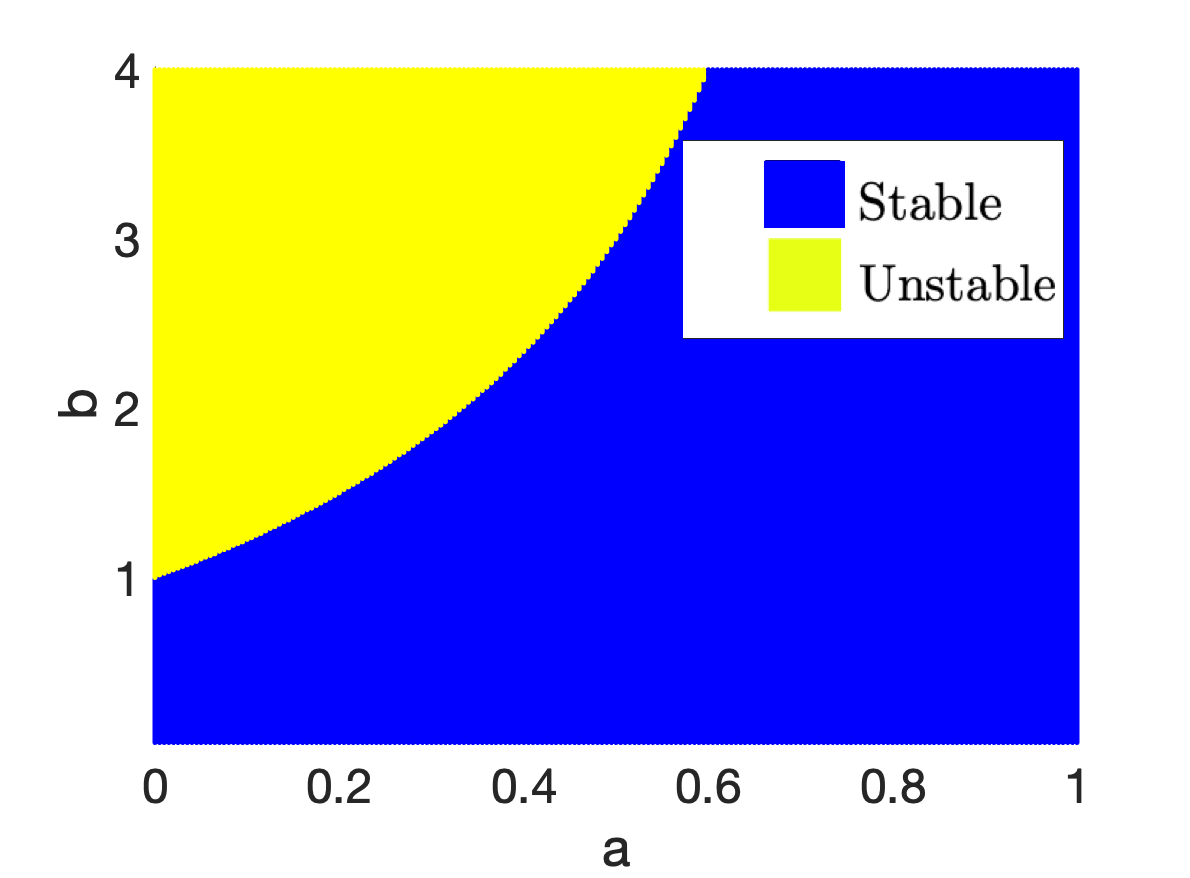
\includegraphics[width=7cm,height = 5cm]{bifgm.png}
        \caption{Bifurcation diagram for spatially homogeneous model, no delay.}
        \label{fig:bifgm}
    \end{subfigure}
    \hfill
    \begin{subfigure}[t]{0.45\textwidth}
        \centering
        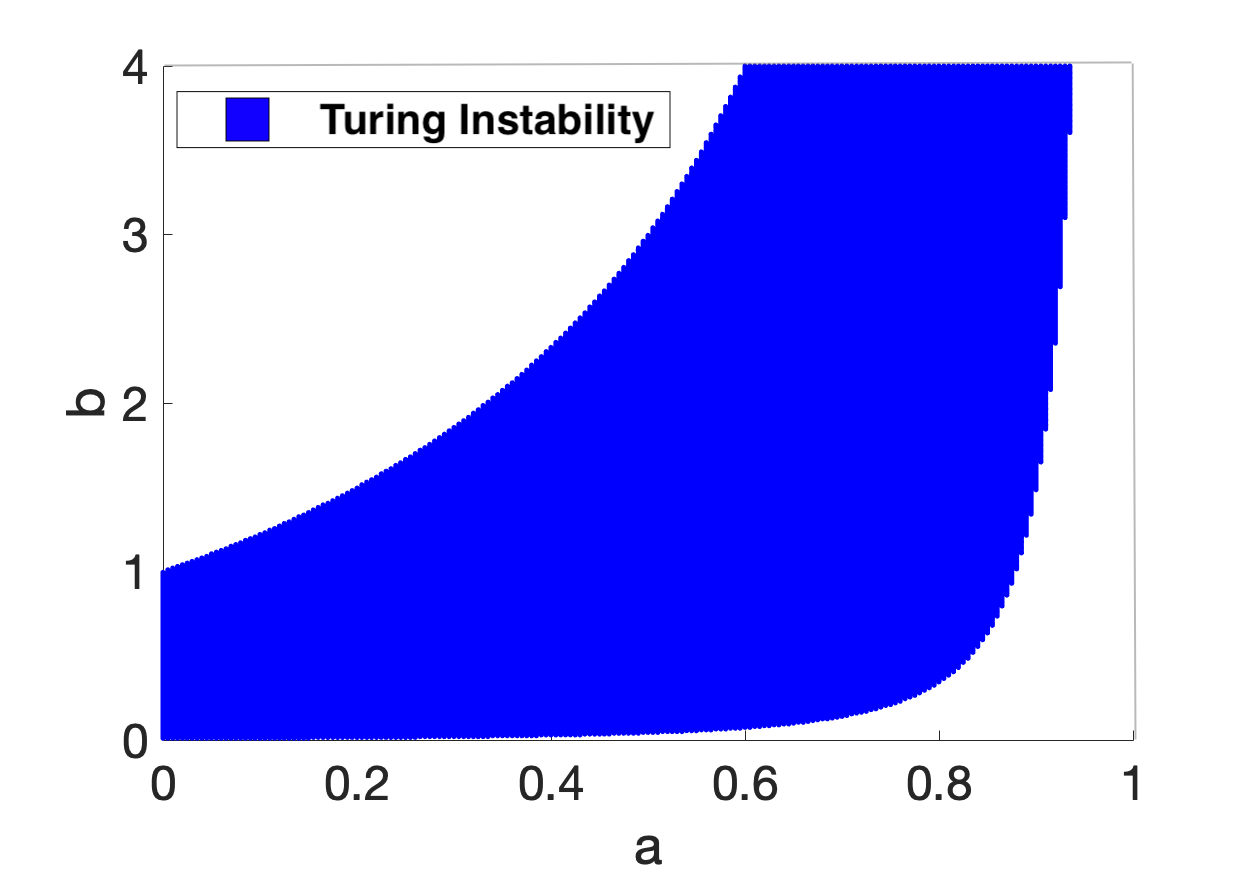
\includegraphics[width=7cm,height = 5cm]{turingspacegm.png}
        \caption{Turing space, no delay. $\epsilon^2=0.001$.}
        \label{fig:turingspacegm}
    \end{subfigure}
    \caption{Conditions \eqref{cond1} and \eqref{cond2} used to plot bifurcation diagram and Turing space for parameters $(a,b)\in[0,1]\times[0,4]$ for GM model.}
    \label{fig:gmspace}
\end{figure}

\section{Linear Analysis}

Using an analogous methodology to that in Chapter \ref{section:fixdel}, we take perturbations $u=u_\star+\delta\xi(x,t)$ and $v=v_\star+\delta\eta$ for $|\delta|\ll1$. The linearised dynamics of \eqref{fadai1} and \eqref{fadai2} are then respectively given by equations \eqref{linf1} and \eqref{linf2}.

\begin{multicols}{2}
\begin{equation}\label{linf1}
    \left.\begin{split}
\frac{\partial \xi}{\partial t}&=\frac{\epsilon^2}{L^2}\frac{\partial^2 \xi}{\partial x^2}-b\xi+2\frac{u_\star}{v_\star}\hat{\xi}-\frac{u_\star^2}{v_\star^2}\hat{\eta},\\
\frac{\partial \eta}{\partial t}&=\frac{1}{L^2}\frac{\partial^2 \eta}{\partial x^2}+2u_\star\hat{\xi}-\eta;
\end{split}\right\}
\end{equation}\break
\begin{equation}
    \left.\begin{split}
\frac{\partial \xi}{\partial t}&=\frac{\epsilon^2}{L^2}\frac{\partial^2 \xi}{\partial x^2}-b\xi+2\frac{u_\star}{v_\star}\hat{\xi}-\frac{u_\star^2}{v_\star^2}\eta,\\
\frac{\partial \eta}{\partial t}&=\frac{1}{L^2}\frac{\partial^2 \eta}{\partial x^2}+2u_\star\hat{\xi}-\eta.\label{linf2}
\end{split}\right\}
\end{equation}
\end{multicols}
with $\hat{\xi}=\xi(x,t-\tau)$ and $\hat{\eta}=\eta(x,t-\tau)$. Substituting into \eqref{linf1} and \eqref{linf2} an ansatz of the form $\begin{pmatrix}\xi\\ \eta\end{pmatrix}=\begin{pmatrix}\xi_0e^{\lambda_kt}\cos(k\pi x)\\\eta_0e^{\lambda_kt}\cos(k\pi x)\end{pmatrix}$ and simplifying, yields a homogeneous system for $(\xi_0,\eta_0)^T$ for each set of linearised dynamics. Finding non-trivial solutions for these systems results in characteristic equations, which can be solved. The charactersitic equations, $\mathcal{D}_k=0$ and $\hat{\mathcal{D}}_k=0$, for the linearised dynamics in \eqref{linf1} and \eqref{linf2} respectively are given by equations \eqref{characf1} and \eqref{characf2}.
\begin{align}\label{characf1}
\mathcal{D}_k&=\lambda_k^2+\alpha_k\lambda+\beta_k+(\gamma_k\lambda_k+\delta_k)e^{-\lambda_k\tau}+\chi_ke^{-2\lambda_k\tau}=0,\\
\hat{\mathcal{D}}_k&=\lambda_k^2+\alpha_k\lambda+\beta_k+(\gamma_k\lambda_k+(\chi_k+\delta_k))e^{-\lambda_k\tau}=0.\label{characf2}
\end{align}
The coefficients for these characteristic equations are given by
\begin{equation}
    \begin{split}
\alpha_k&=\left(\frac{\epsilon^2}{L^2}+\frac{1}{L^2}\right)k^2\pi^2+b+1,\\
\beta_k&=\left(\frac{\epsilon^2}{L^2}\pi^2k^2+b\right)\left(\frac{1}{L^2}\pi^2k^2+1\right),\\
\gamma_k&=-2\frac{u_\star}{v_\star},\\
\delta_k&=-2\frac{u_\star}{v_\star}\left(\frac{1}{L^2}k^2\pi^2+1\right),\\
\chi_k&=2\frac{u_\star^3}{v_\star^2}.
    \end{split}
\end{equation}

The roots of \eqref{characf1} and \eqref{characf2} can thus be solved, and plots of $\max_k(\Re(\lambda_k))$ across the parameter plane $(a,b)\in[0,1]\times[0,4]$ for each of the models \eqref{fadai1} and \eqref{fadai2}, can be generated. Figures \ref{fig:fad1} and \ref{fig:fad2} show these results for varying $\tau$, where we have also added the contour lines of $\Re(\lambda_0)=0$ and $\max_k(\Re(\lambda_k))=0$ to indicate the Turing space.
\begin{figure}[H]
    \centering
    \begin{subfigure}[t]{0.32\textwidth}
        \centering
        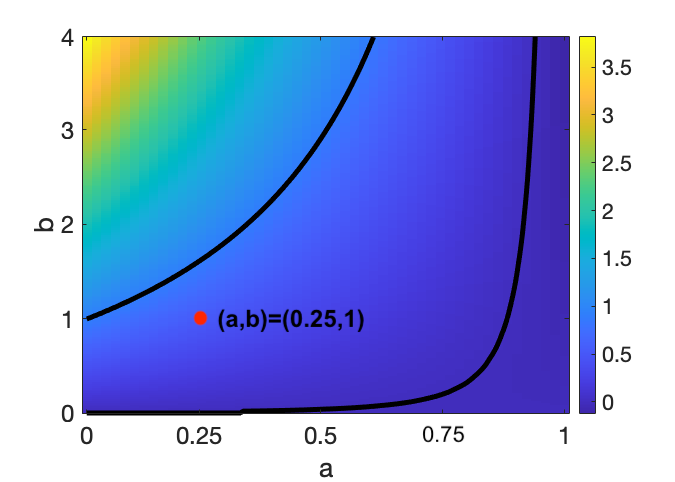
\includegraphics[width=5.5cm,height = 5cm]{f1t0.png}
        \caption{$\tau=0$.}
        \label{}
    \end{subfigure}
    \hfill
    \begin{subfigure}[t]{0.32\textwidth}
        \centering
        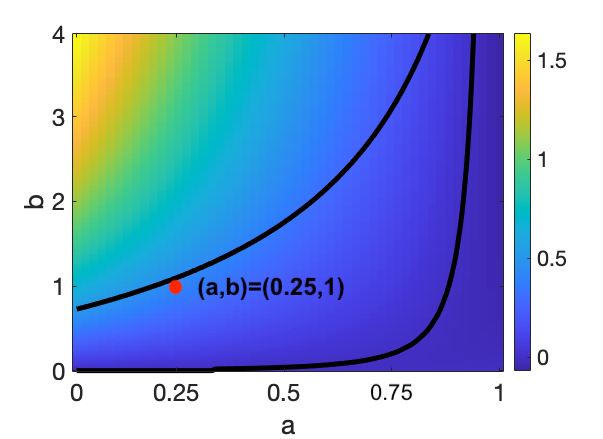
\includegraphics[width=5.5cm,height = 5cm]{f1t02.png}
        \caption{$\tau=0.2$.}
        \label{}
    \end{subfigure}
    \hfill
    \begin{subfigure}[t]{0.32\textwidth}
        \centering
        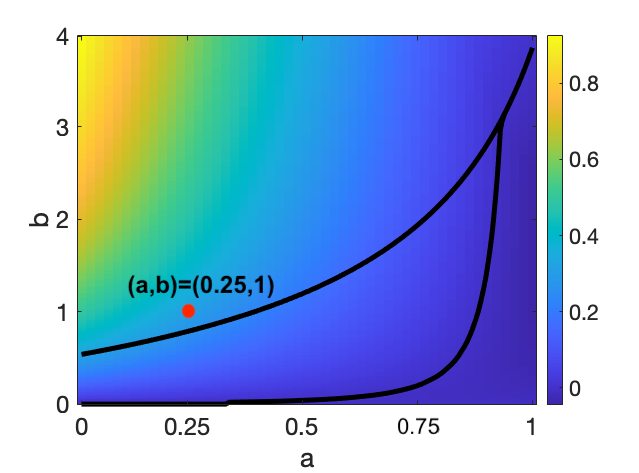
\includegraphics[width=5.5cm,height = 5cm]{f1t05.png}
        \caption{$\tau=0.5$.}
        \label{f}
    \end{subfigure}
    \caption{Result for model in \eqref{fadai1}. $\max_k(\Re(\lambda_k))$ plotted for $(a,b)\in[0,1]\times[0,4]$, with varying $\tau$. $\max_k$ taken over $k\in[0,50]$ for $k\in\mathbb{Z}$. Parameters $\epsilon^2=0.001$ and $L^2=9/2$ used.}
    \label{fig:fad1}
\end{figure}
\begin{figure}[H]
    \centering
    \begin{subfigure}[t]{0.32\textwidth}
        \centering
        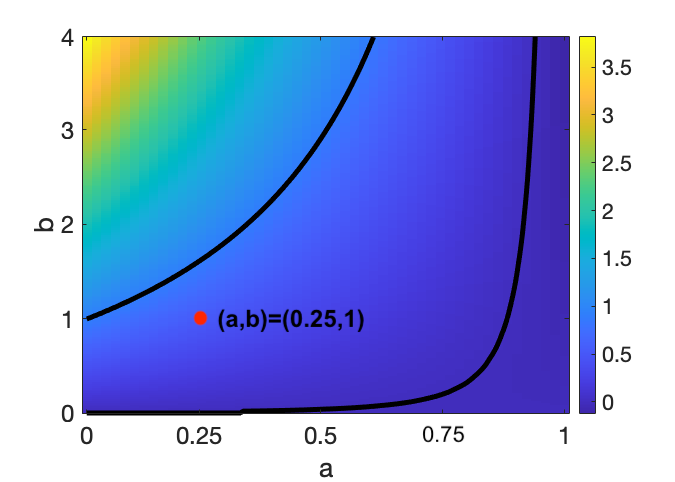
\includegraphics[width=5.5cm,height = 5cm]{f1t0.png}
        \caption{$\tau=0$.}
        \label{}
    \end{subfigure}
    \hfill
    \begin{subfigure}[t]{0.32\textwidth}
        \centering
        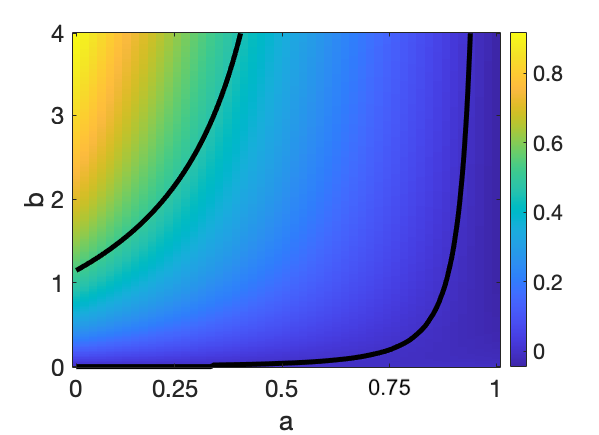
\includegraphics[width=5.5cm,height = 5cm]{f2t05.png}
        \caption{$\tau=0.5$.}
        \label{}
    \end{subfigure}
    \hfill
    \begin{subfigure}[t]{0.32\textwidth}
        \centering
        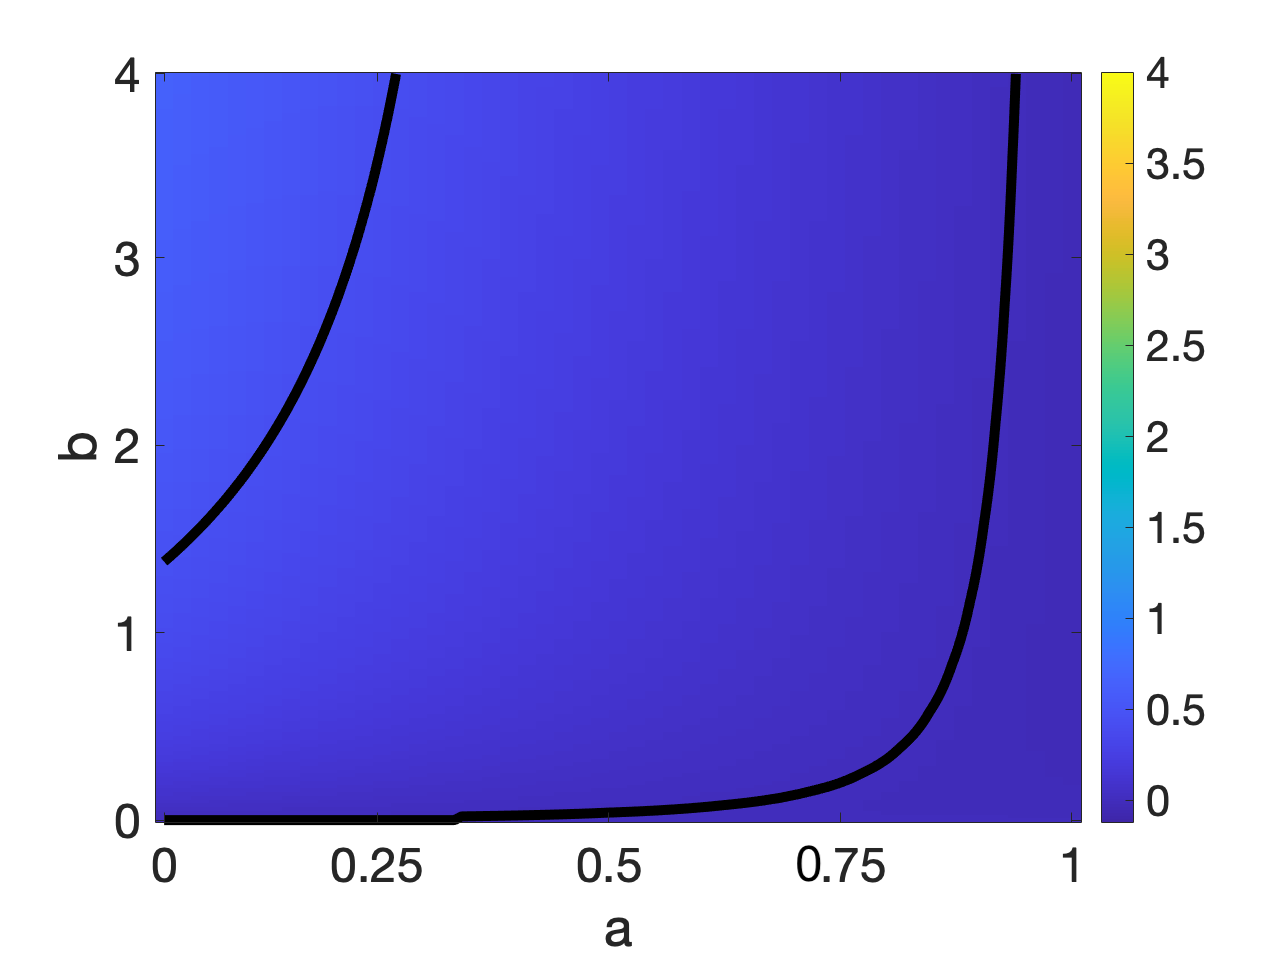
\includegraphics[width=5.5cm,height = 5cm]{f2t08.png}
        \caption{$\tau=0.8$.}
        \label{}
    \end{subfigure}
    \caption{Result for model in \eqref{fadai2}. $\max_k(\Re(\lambda_k))$ plotted for $(a,b)\in[0,1]\times[0,4]$, with varying $\tau$. $\max_k$ taken over over $k\in[0,50]$ for $k\in\mathbb{Z}$. Parameters $\epsilon^2=0.001$ and $L^2=9/2$ used.}
    \label{fig:fad2}
\end{figure}
For the model given in \eqref{fadai1}, where analysis in \cite{fadai1} showed a de-stabilisation of the stable spike solution parameter space with an increasing $\tau$, the results in figure \ref{fig:fad1} show a similar result for Turing instabilities. Namely, the Turing space shrinks for increasing $\tau$. Similarly, \cite{fadai2} showed a stabilising effect of increasing $\tau$ on the stable spike solution parameter space for the model in \eqref{fadai2}, and we find an analogous result for the Turing space, as seen in figure \ref{fig:fad2}. We note here that in all models considered, namely the LI model, and the two GM model variants, the changing size of the Turing space with an increasing $\tau$ is solely dependent on the movement of the curve produced by considering the homogeneous characteristic equation (when $k=0$). This similarity could suggest a particular mechanism by which stabilising or de-stabilising effects of time delay on the Turing space arise.

Finally, through numerical simulations, we present a linearly increasing relationship between time delay and time-to-pattern for both variants of the GM model. For the model in \eqref{fadai1}, as a result of the shrinking Turing space, we only consider small $\tau\in[0.1,1]$, varied at regular intervals of $0.1$. For the model in \eqref{fadai2}, we consider $\tau\in[1,16]$, varied at regular intervals of $1$. Using a similar methodology to compute time-to-pattern as in Chapter 2, we set an initial perturbation from the steady state as $\sigma_{\text{IC}}=0.01$, and a threshold value of $2$. These larger values were chosen to improve computational time, and should not impact the relationship we see. The figures for the time-to-pattern results for \eqref{fadai1} and \eqref{fadai2} can be seen in \ref{fig:fadlin}, where a linear relationship can be deduced for both models.

\begin{figure}[H]
    \centering
    \begin{subfigure}[t]{0.45\textwidth}
        \centering
        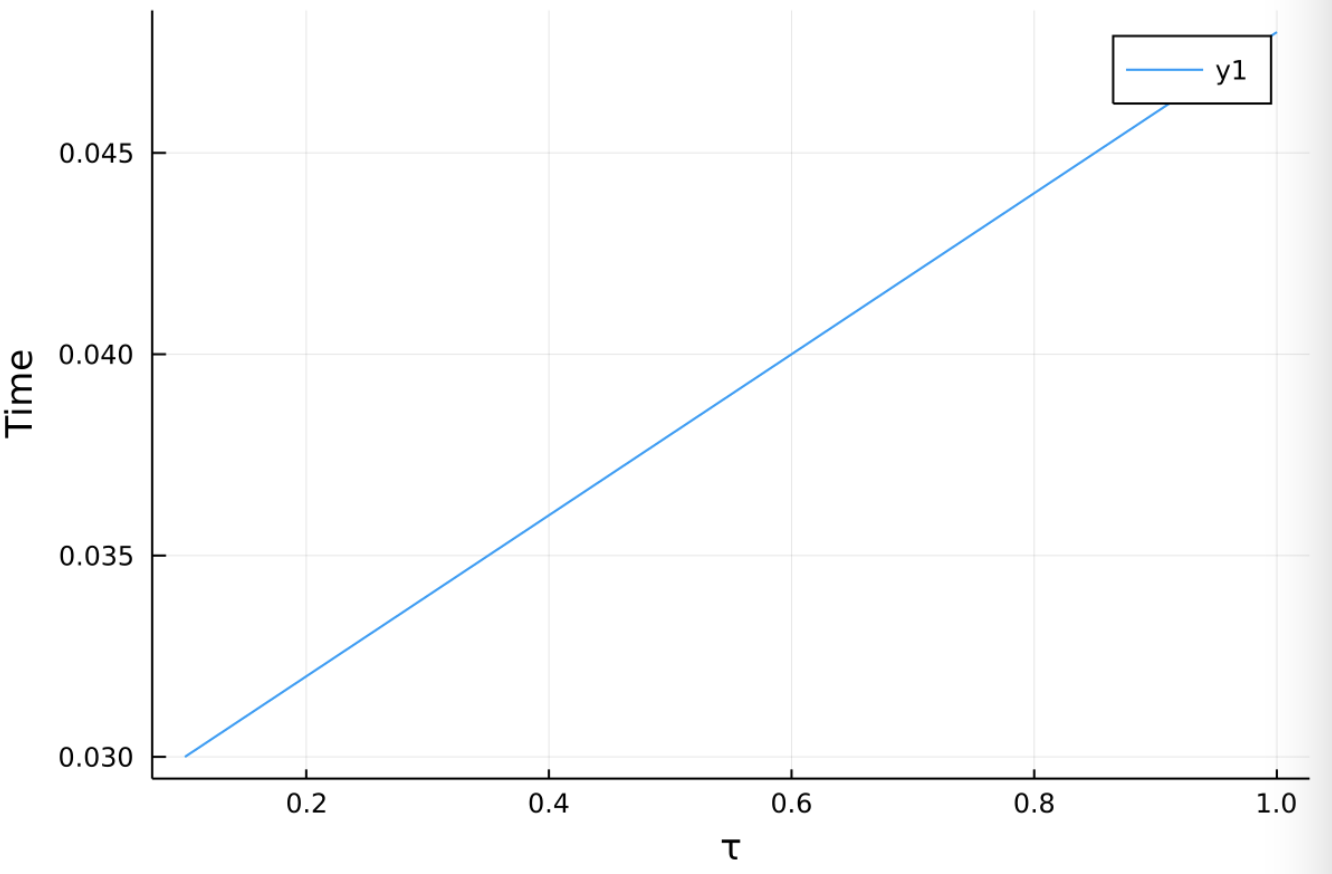
\includegraphics[width=6cm,height = 5cm]{fad2lin.png}
        \caption{Model given in \eqref{fadai1}. $\tau\in[0.1,1]$ varied at intervals of $0.1$.}
        \label{}
    \end{subfigure}
    \hfill
    \begin{subfigure}[t]{0.45\textwidth}
        \centering
        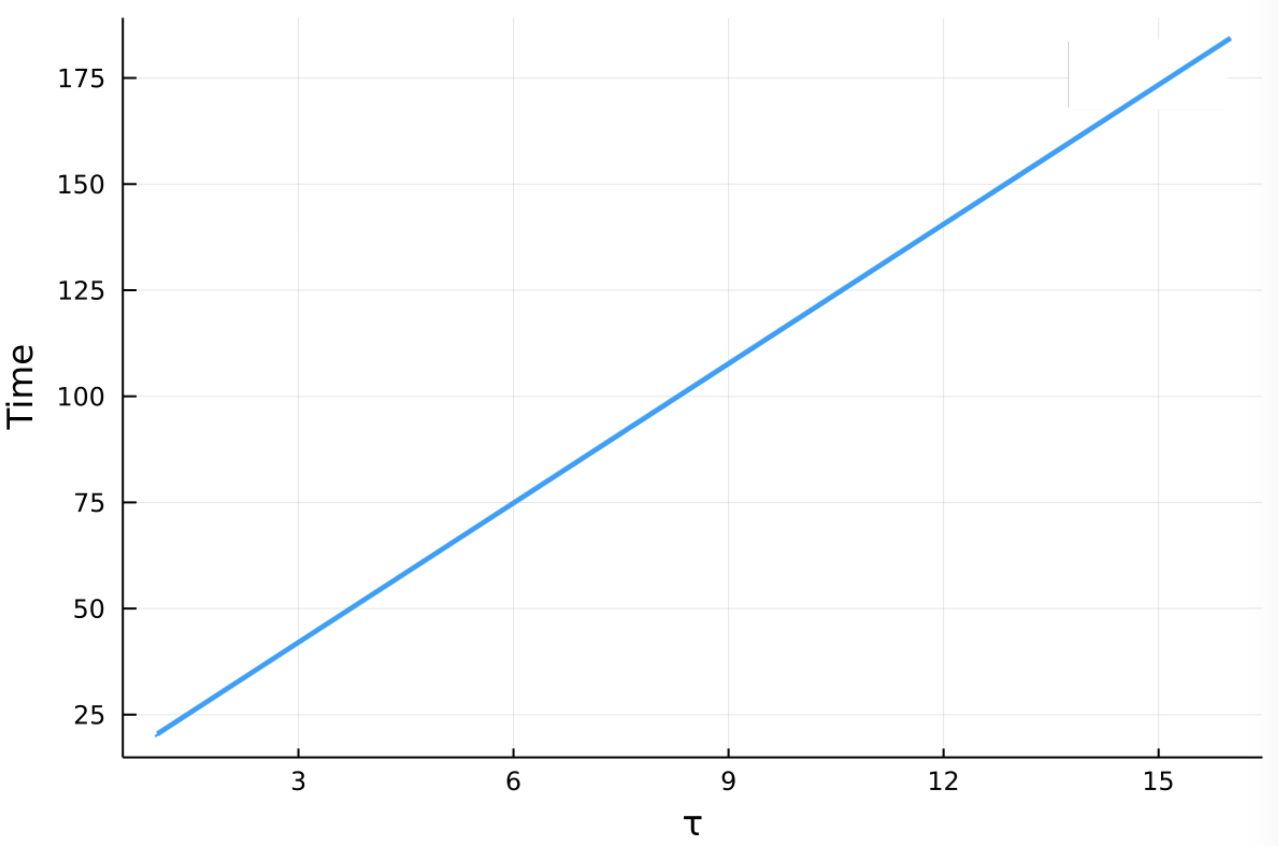
\includegraphics[width=6cm,height = 5cm]{gmlin1.png}
        \caption{Model given in \eqref{fadai2}. $\tau\in[1,16]$ varied at intervals of $1$.}
        \label{}
    \end{subfigure}
    \caption{Time-to-pattern results for the two GM variants given in \eqref{fadai1} and \eqref{fadai2}. Initial random perturbation given with $\sigma_{\text{IC}}=0.01$, and threshold value given as $2$.}
    \label{fig:fadlin}
\end{figure}
